\section{Overall System Architecture}
\label{sec:architecture}

\subsection{Architectural Paradigm}
Research Rover is designed following a modular, five-tier layered software architecture. The platform enforces strict separation of concerns, decoupling user presentation, API dispatching, scientific domain computation, local persistence, and external data provider communications.

\begin{figure}[H]
\centering
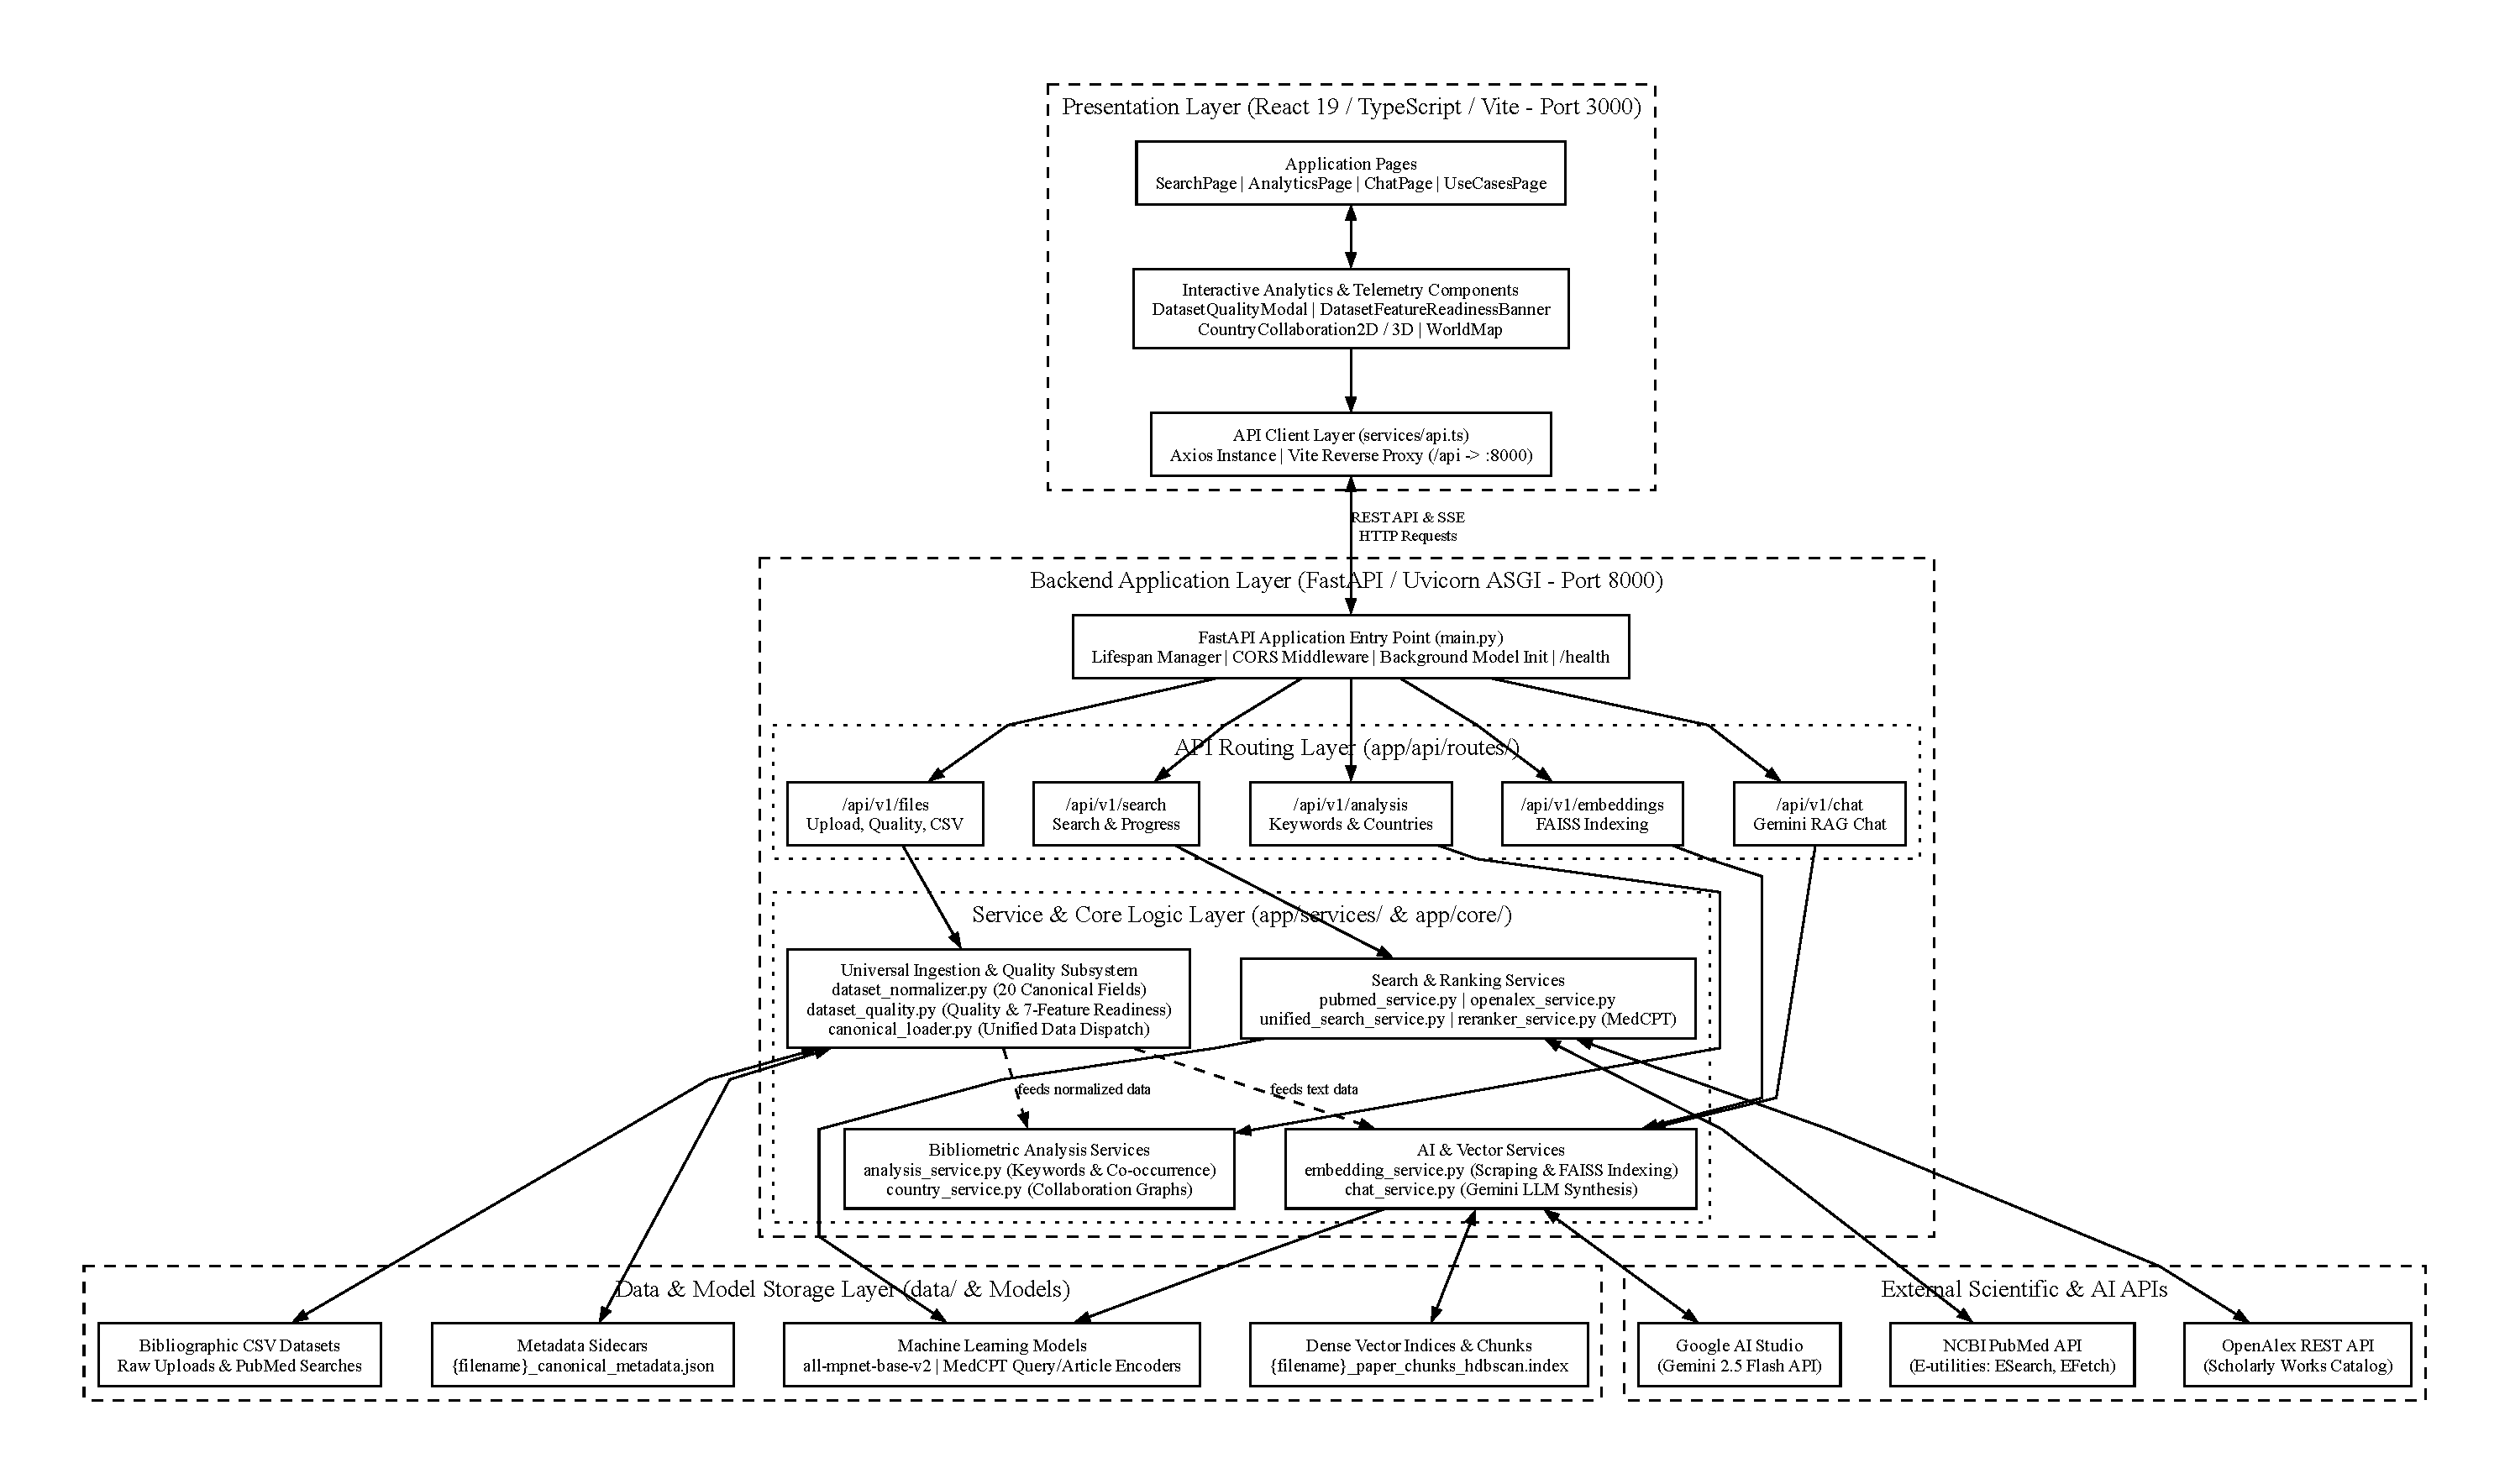
\includegraphics[width=0.95\textwidth]{figures/system_architecture.pdf}
\caption{Overall Multi-Tier System Architecture of Research Rover}
\label{fig:system_architecture}
\end{figure}

As depicted in Figure~\ref{fig:system_architecture}, the system consists of five cohesive layers:

\subsection{Detailed Architectural Layers}

\subsubsection{1. Presentation Layer (Frontend SPA)}
The presentation tier is implemented as a client-side Single-Page Application (SPA) utilizing React 19 and TypeScript. It includes:
\begin{itemize}
    \item \textbf{Routing and View Pages:} Managed by React Router v7, presenting the Search Portal (\texttt{SearchPage.tsx}), Bibliometric Analytics Dashboard (\texttt{AnalyticsPage.tsx}), Conversational RAG Interface (\texttt{ChatPage.tsx}), and Project Use-Case Demonstrations (\texttt{UseCasesPage.tsx}).
    \item \textbf{Diagnostic Components:} Including the \texttt{DatasetQualityModal.tsx} for inspecting uploaded dataset health, and \texttt{DatasetFeatureReadinessBanner.tsx} for informing users of analytical feature readiness.
    \item \textbf{Visualisation Engines:} Integrating Three.js and ForceGraph for dynamic two-dimensional and three-dimensional international research collaboration topologies.
    \item \textbf{API Client Module:} Encapsulated within \texttt{frontend/src/services/api.ts}, utilizing Axios with request timeouts and automatic payload transformation.
\end{itemize}

\subsubsection{2. API Dispatch and Routing Layer (FastAPI Backend)}
The entry point of the server application is \texttt{backend/main.py}, operating under the Uvicorn ASGI server. This layer manages:
\begin{itemize}
    \item \textbf{Cross-Origin Resource Sharing (CORS):} Configured via FastAPI \texttt{CORSMiddleware} to allow seamless communication between the frontend client and backend API.
    \item \textbf{Modular Route Controllers:} Subdividing incoming requests across six route controllers: \texttt{search.py}, \texttt{files.py}, \texttt{analysis.py}, \texttt{embeddings.py}, \texttt{chat.py}, and \texttt{system.py}.
    \item \textbf{Lifespan Task Execution:} Managing background thread pools for non-blocking model pre-loading.
\end{itemize}

\subsubsection{3. Business Logic and Service Layer}
This layer houses the analytical, retrieval, and machine learning logic:
\begin{itemize}
    \item \textbf{Search Subsystem:} Dispatches queries to PubMed and OpenAlex, standardizes responses, and applies MedCPT zero-shot bi-encoder re-ranking.
    \item \textbf{Universal Ingestion Subsystem:} Executes four-tier header matching, data cleaning, multi-attribute quality scoring, and seven-feature readiness verification.
    \item \textbf{Bibliometric Analytics Subsystem:} Extracts author country affiliations, builds co-occurrence networks, and calculates keyword frequency matrices.
    \item \textbf{Vector and AI Subsystem:} Chunks texts, computes 768-dimensional embeddings via Sentence Transformers, indexes vectors using FAISS, and synthesizes answers via Google Gemini.
\end{itemize}

\subsubsection{4. Persistence and Storage Layer}
All persistent data is organized within the root \texttt{data/} directory:
\begin{itemize}
    \item \textbf{Tabular Datasets:} Raw and normalized research paper CSV files.
    \item \textbf{Metadata Sidecars:} Dedicated \texttt{*\_canonical\_metadata.json} sidecar files storing quality scores, field mappings, and feature readiness telemetry.
    \item \textbf{Vector Indexes:} FAISS binary indexes (\texttt{*\_paper\_chunks\_hdbscan.index}) and associated chunk mapping files.
    \item \textbf{Full-Text Cache:} JSON mappings correlating paper DOIs with scraped full-text content.
\end{itemize}

\subsubsection{5. External Research and Intelligence Providers}
Research Rover interfaces securely with external academic and computational services:
\begin{itemize}
    \item \textbf{NCBI E-utilities API:} Provides access to over 35 million biomedical citations via \texttt{esearch.fcgi} and \texttt{efetch.fcgi}.
    \item \textbf{OpenAlex REST API:} Provides multidisciplinary scholarly graph data across global institutions.
    \item \textbf{Google AI Studio (Gemini 2.5 Flash):} Powers advanced natural language understanding and context synthesis.
\end{itemize}
